\documentclass{beamer}

\usepackage[utf8]{inputenc}
\usepackage{lmodern}
\usepackage{xfrac}

\usetheme{CambridgeUS}
\usecolortheme{seagull}
\setbeamertemplate{headline}{}
\setbeamertemplate{caption}{\raggedright\insertcaption\par}

\title{PageRank}
\author[A. L. R. Teixeira, G. Zambonin]
{Antonio Luiz Rosa Teixeira\texorpdfstring{\\ Gustavo Zambonin}{}}
\institute[]{\newline
Universidade Federal de Santa Catarina \\
Departamento de Informática e Estatística \\
INE5413 - Grafos}
\date{}

\begin{document}

\begin{frame}
    \titlepage
\end{frame}

\begin{frame}
    \frametitle{Introdução}
    \begin{itemize}
        \item Desenvolvido por Page e Brin em 1996
        \begin{itemize}
            \item Parte do motor de busca da Google desde 1998
        \end{itemize}
        \item Classificação de uma página na web, independente do seu conteúdo
        \item Entretanto, depende do número de links que apontam para ela
        \item Abrange diversas áreas da matemática
        \begin{itemize}
            \item Teoria de grafos
            \item Probabilidade e estatística
            \item Álgebra linear
        \end{itemize}
        \item Definições genéricas e aplicáveis a qualquer grafo
    \end{itemize}
\end{frame}

\begin{frame}
    \frametitle{Motivação}
    \begin{itemize}
        \item Motores de busca prévios utilizavam
        heurísticas facilmente manipuláveis
        \begin{itemize}
            \item Tamanho do URL
            \item Conteúdo bruto da página
            \item Título da página
        \end{itemize}
        \item Método mais eficiente de relevar páginas de
        acordo com as palavras-chave da pesquisa
        \item Evitar meios artificiais de inflação de popularidade
    \end{itemize}
\end{frame}

\begin{frame}
    \frametitle{Modelagem}
    \begin{columns}[T]
        \begin{column}{.55\textwidth}
            \begin{itemize}
                \item Assume-se um `navegador' de páginas, que clicará em
                links aleatoriamente, até que isto seja impossível
                \item Possível representar relações entre páginas como um
                grafo direcionado
                \item Seja um grafo G(V, A), então:
                \begin{center}
                    V = $\{$p $\mid$ p é uma página da web$\}$ \\
                    A = $\{$($r_1, r_2$) $|$ $r_2$ referencia
                        $r_1$ por um \textit{hyperlink}$\}$
                \end{center}
            \end{itemize}
        \end{column}
        \begin{column}{.4\textwidth}
        \begin{figure}
            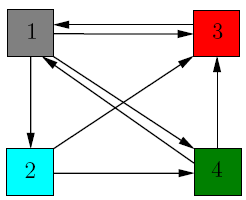
\includegraphics[scale=0.45]{pr_1}
            \caption{\tiny{Supondo uma rede com apenas quatro páginas e
            referências entre estas, tem-se o grafo acima.}}
        \end{figure}
        \end{column}
    \end{columns}
\end{frame}

\begin{frame}
    \frametitle{Resolução}
    \begin{itemize}
        \item Cada página deve transferir sua `importância' $\frac{1}{k}$ para
        seus sucessores
        \begin{itemize}
            \item $k =$ grau de emissão do vértice
            \item Processo de valoração de arestas
        \end{itemize}
        \item Tem-se uma matriz de transições do grafo
        \item Para o exemplo anterior (cada coluna representa uma página):
        \begin{equation*}
            \begin{bmatrix}
                0 & 0 & 1 & \sfrac{1}{2} \\
                \sfrac{1}{3} & 0 & 0 & 0 \\
                \sfrac{1}{3} & \sfrac{1}{2} & 0 & \sfrac{1}{2} \\
                \sfrac{1}{3} & \sfrac{1}{2} & 0 & 0
            \end{bmatrix} \stackrel{\text{Av = $\lambda$v}}{\approx}
            1 \times \begin{bmatrix}
                0.7210 \\ 0.2403 \\ 0.5408 \\ 0.3605
            \end{bmatrix}
        \end{equation*}
        \item O autovetor denota a probabilidade das páginas serem visitadas
    \end{itemize}
\end{frame}

\begin{frame}
    \frametitle{Problemas}
    \begin{itemize}
        \item Se $k = 0$ para uma página qualquer, então a página não terá
        importância alguma, no modelo acima
        \begin{figure}
            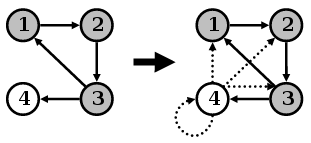
\includegraphics[scale=0.35]{pr_2}
            \caption{\tiny{A página `4', um sumidouro, deve possibilitar a
            navegação para o resto do grafo}}
        \end{figure}
        \item Se o grafo é desconexo, como mover entre componentes?
        \begin{itemize}
            \item Considerar que o `navegador' aleatório pode se cansar de
            clicar e querer trocar de página de outro modo
        \end{itemize}
        \item Adicionar um fator probabilístico que lida com estes cenários
    \end{itemize}
\end{frame}

\begin{frame}
    \frametitle{Aplicações}
    \begin{itemize}
        \item Métrica para profundidade e extensão de \textit{web crawling}
        \item Funções mais importantes no kernel Linux
        \item Recomendação de seguidores no Twitter, produtos na Amazon e
        filmes no Netflix
        \item Impacto científico de pesquisadores e artigos
        \item Sistema de ranking entre times ou atletas em esportes
        \item Encontrar genes correlacionados de acordo com um certo critério
        \item Predição de fluxo de tráfego e pessoas em um sistema urbano
        \item Ranking de isomorfismos de grafos
    \end{itemize}
\end{frame}

\begin{frame}
    \frametitle{Referências}
    \begin{thebibliography}{10}
  \beamertemplatearticlebibitems
  \bibitem{wills}
    R.S.~Wills.
    \newblock Google’s PageRank: The Math Behind the Search Engine
    \newblock {\em The Matematical Intelligencer}, 28(4):6--10, 2006.
  \beamertemplatearticlebibitems
  \bibitem{page}
    L.~Page, S.~Brin, R.~Motwani, T.~Winograd.
    \newblock The PageRank Citation Ranking: Bringing Order to the Web.
    \newblock {\em Stanford InfoLab}, 1999.
  \beamertemplatearticlebibitems
  \bibitem{gleich}
    D.F.~Gleich.
    \newblock PageRank beyond the Web
    \newblock {\em SIAM Review}, 57(3):321--363, 2015.
  \beamertemplateonlinebibitems
  \bibitem{tanase}
    R.~Tanase, R.~Radu.
    \newblock PageRank Algorithm - The Mathematics of Google Search
    \newblock
    \href{http://www.math.cornell.edu/~mec/Winter2009/RalucaRemus/Lecture3/lecture3.html}
    {Lecture 3}, 2009.
  \end{thebibliography}
\end{frame}

\end{document}
